


\def \fgw {1.77in}



\begin{figure}[t]

%\centerline{

%}



\centerline{
\hmina
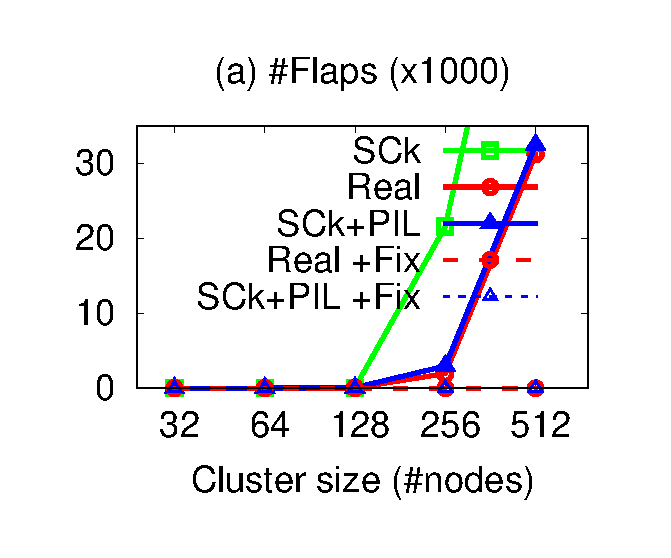
\includegraphics[width=\fgw]{F/accu/eps/flap}
\hminb
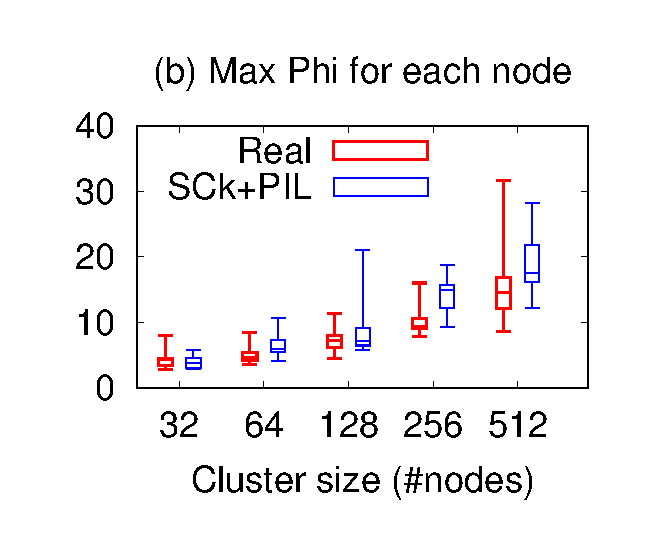
\includegraphics[width=\fgw]{F/accu/eps/phi}
\hmina
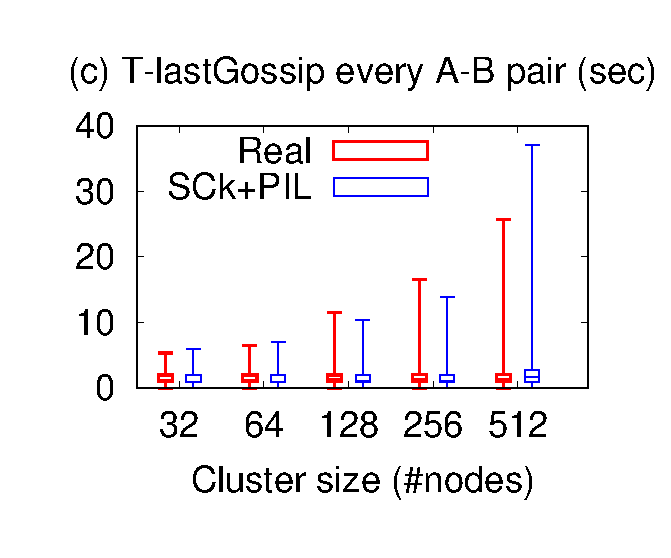
\includegraphics[width=\fgw]{F/accu/eps/hb}
\hminb
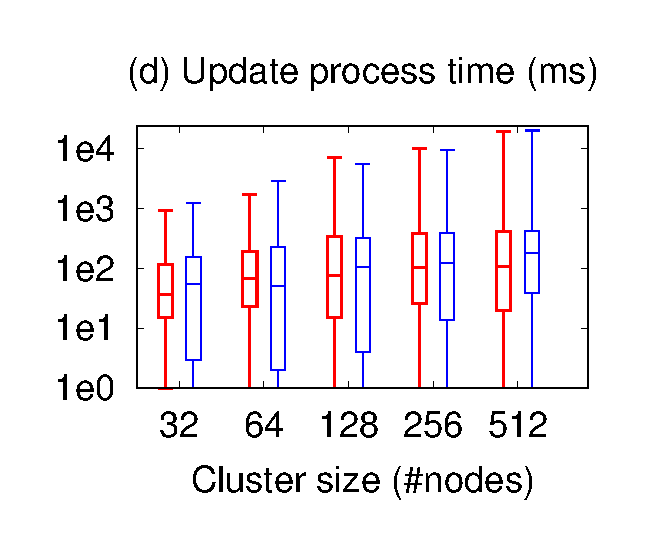
\includegraphics[width=\fgw]{F/accu/eps/proc-log}
}

\vfive % orphan : we have extra space on page 10

%\centerline{
%\hmina
%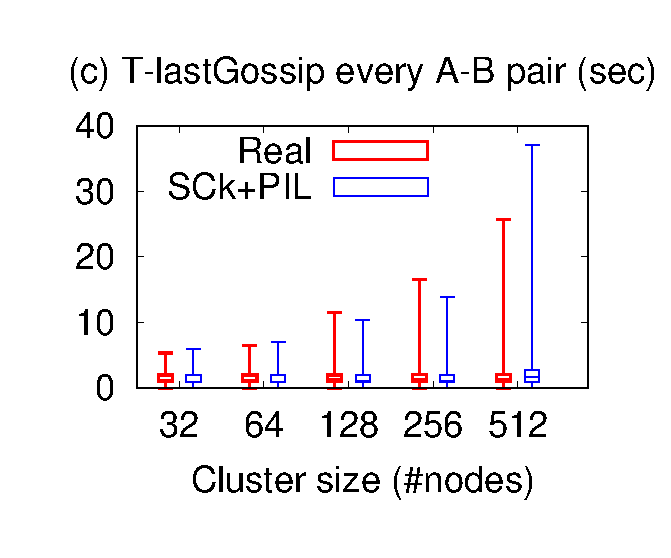
\includegraphics[width=\fgw]{F/accu/eps/hb}
%\hminb
%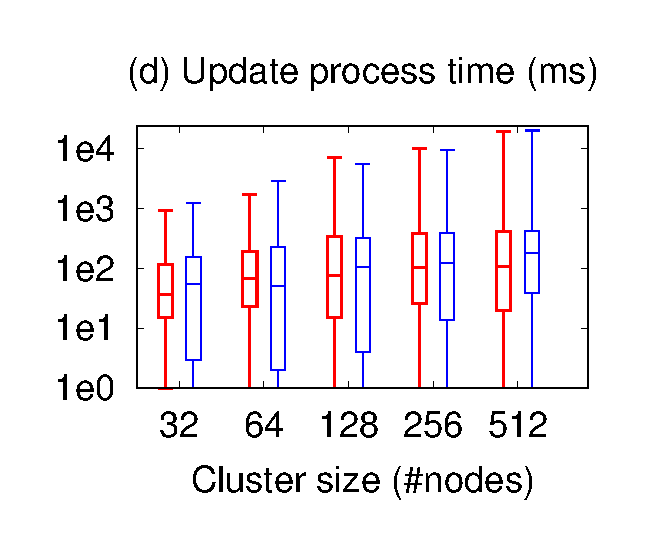
\includegraphics[width=\fgw]{F/accu/eps/proc-log}
%}

%\centerline{
%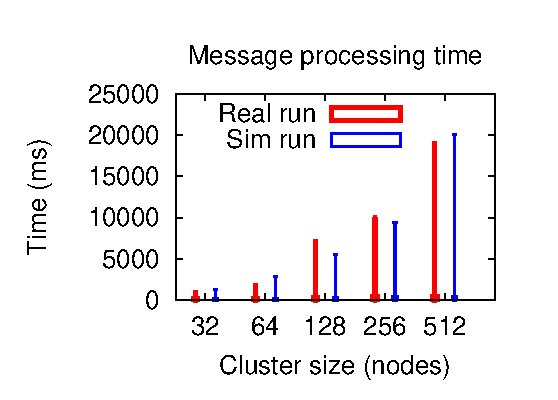
\includegraphics[width=\fgw]{F/accu/eps/proc}
%\includegraphics[width=\fgw]{F/accu/eps/hop}
%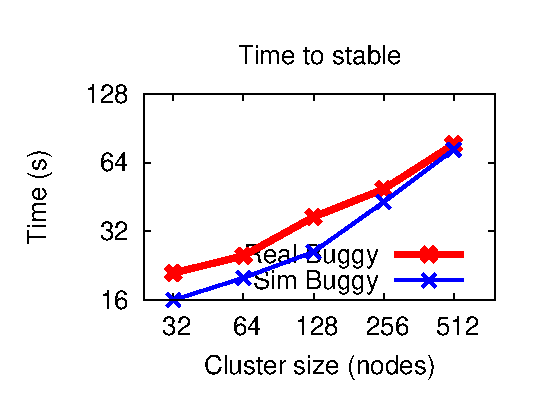
\includegraphics[width=\fgw]{F/accu/eps/stable}
%}

\vminten
\mycaption{fig-accu}{Accuracy in reproducing \caone (\sec\ref{eval-accu})}{The 
figures represent the metrics presented in Figure \ref{fig-form},
measured in real deployment (``Real'') and \sck with
different cluster sizes (32, 64, 128, 256, and 512).
Figure title represents the y-axis.}
\vminfive
\end{figure}




\if 0

\hsg{ b - 512
 c - 41295431
 d - 24335
recap, exampe, how many data points.
}

% \includegraphics[width=\fgw]{F/graphs/ca-6127/tsilent_99}
% \includegraphics[width=\fgw]{F/graphs/ca-6127/avgtsilent_99}
\includegraphics[width=\fgw]{F/graphs/ca-6127/avgtsilent}
\includegraphics[width=\fgw]{F/graphs/ca-6127/hop}
\includegraphics[width=\fgw]{F/graphs/ca-6127/hop}
\includegraphics[width=\fgw]{F/graphs/ca-6127/proctime}
\includegraphics[width=\fgw]{F/graphs/ca-6127/proctime_99}
\includegraphics[width=\fgw]{F/graphs/ca-6127/commit}
\includegraphics[width=\fgw]{F/graphs/ca-6127/commit_99}
\includegraphics[width=\fgw]{F/graphs/ca-6127/profiling}
\includegraphics[width=\fgw]{F/graphs/ca-6127/table}
\includegraphics[width=\fgw]{F/graphs/ca-6127/table_med}
\fi
